% !Mode:: "TeX:UTF-8" 

\BiChapter{感知融合与模型决策}{3}\label{chpt-3}
% 本章分别从目标识别、光学字符识别、图像分类三个方面介绍感知提取模型。感知融合结果作为第~\ref{chpt-4}~章决策模型的输入基础,
% 下文分别从状态、动作、奖励特征提取三个方面进行介绍,
% 相关实验结果在~\ref{sec-exp-detect}~中展示。
\BiSection{感知模型}{}\label{sec-perceptron}
\BiSubsection{目标识别模型}{}
本文使用YOLO系列模型作为本次目标识别模型,分别尝试了YOLOv5\upcite{YOLOv5}和YOLOv8\upcite{YOLOv8}作为目标识别器,
下面分别对其模型架构改进进行介绍:

YOLOv5主要是对YOLOv4\upcite{YOLOv4}模型进行了少许改进,YOLOv4模型在Backbone部分(初步特征提取)的主要改进
是使用了基于跨阶段部分网络(Cross Stage Partial Networks, CSPNet)\upcite{CSPNet}
结构的DarkNet\upcite{YOLOv3}并在输出特征时使用空间金字塔池化(Spatial Pyramid Pooling,SPP)\upcite{SPP}对特征进行不同尺度上的提取,
在Neck部分(进一步特征提取)中使用了路径聚合网络(Path Aggregation Network, PANet)\upcite{PANet},结合特征金字塔与路径压缩,
缩短了较低层与最顶层特征之间的信息路径,能够有效进行特征融合。

而YOLOv8模型结构上仍然使用CSP和SPP进行特征提取,相对YOLOv5使用了更多的工程优化方法对模型预测速度进行大幅优化,
Head部分(预测框输出)则重新回到YOLOv1\upcite{YOLO}无锚框预测的方法,使预测框不再受到锚框约束。

ByteTrack\upcite{ByteTrack}是一种基于Kalman滤波\upcite{KalmanFilter}的多目标跟踪(Multiple Object Tracking, MOT)算法,
首先需要分别对不同边界框作为跟踪对象,建立独立的线性运动方程,通过Kalman滤波结合之前帧的追踪信息,
以递归的方式给出目标边界框在当前时刻下的位置预测,再通过计算IOU定位当前帧下跟踪对象的位置。
与传统MOT算法不同的是,
ByteTrack尝试利用滤波预测的方法,从更低的置信度对应的边界框中找到可能被忽略的跟踪边界框,
从而恢复可能因遮挡等原因被低估的边界框。

\BiSubsection{光学字符识别模型}{}
PaddleOCR\upcite{PPOCR}是百度公司研发并开源的一个基于PaddlePaddle框架的光学字符识别(Optical Character Recognition, OCR)
系统,PaddleOCR提供了一整套从图像预处理到文字识别的方案,其模型架构主要分为如下两个模块:
\begin{enumerate}
  \item 文本检测模块:使用ResNet\upcite{ResNet}、MobileNet\upcite{MobileNet}等经典的卷积神经网络作为特征提取网络,使用特征金字塔网络(Feature Pyramid Networks,FPN)\upcite{FPN}等方法来融合多尺度特征,
  使用可微分二值化(Differentiable Binarization,DB)\upcite{DB}等方法来预测文本框。
  \item 文本识别模块:使用卷积循环神经网络(Convolutional Recurrent Neural Networks, CRNN)\upcite{CRNN}提取文字区域的特征,
  首先使用卷积网络对图像进行特征提取,再使用Bi-LSTM\upcite{BiLSTM}等序列模型来捕捉字符之间的依赖关系,
  最后使用CTC(Connectionist Temporal Classification)\upcite{CTC}作为文字序列的损失函数。
\end{enumerate}

\BiSubsection{图像分类模型}{}
本毕设的图像分类模型使用ResNet结构,其核心思想是通过引入短连接(Shortcut Connections),
使得网络可以直接学习残差(Residual),从而更容易学习到恒等映射,
缓解深度神经网络中梯度消失的问题。具体来说,ResNet使用残差块(Residual Block)来实现上述操作,
残差块由两部分构成,卷积层:卷积变换$F_W(\cdot)$、批归一化(Batch Normalization, BN)\upcite{BN}以及ReLU激活函数;
残差连接:将输入直接加在卷积层的输出结果上。残差块结构可以表示为
\begin{equation}
  y = \sigma(\text{BN}(F_W(x))) + x
\end{equation}
其中$x$为输入图像特征,$y$为输出图像特征,$F_W$是以卷积核$W$的卷积变换,BN为批归一化操作,$\sigma(x)=\frac{x+|x|}{2}$为ReLU函数。

\BiSection{感知特征提取}{}
在感知特征提取中,本文将同时用到上述三种模型作为一阶段图像特征提取,分别可以得到当前时刻下三个预处理信息:
剩余时间(OCR)、竞技场中的预测框(YOLO)、当前手牌及总圣水(图像分类器)。
下面将介绍特征提取器的设计方法,可以将预处理信息进一步转化为决策模型的输入信息,它们分别为
环境状态信息提取(State)、执行动作信息提取(Action)和环境奖励信息提取(Reward)。
\begin{wrapfigure}[13]{r}{.5\textwidth} % 文字环绕行数为13行, 图片靠右 (l为靠左), 图片占0.5的行宽
  \centering
  \vspace{-1ex}
  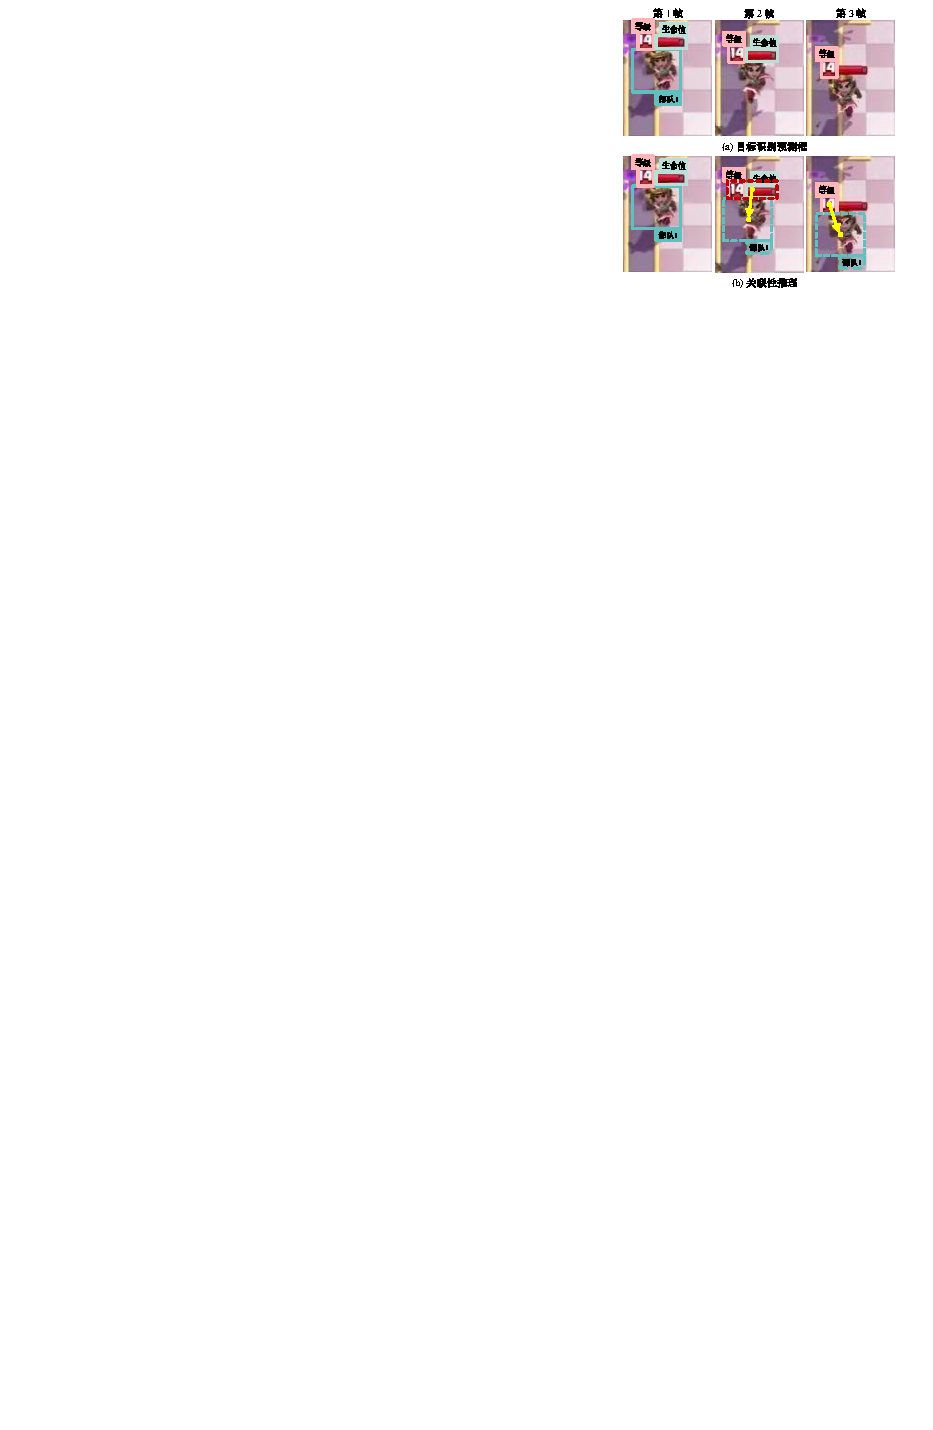
\includegraphics[width=.5\textwidth]{perceptron_improve.pdf}
  \vspace{-1ex}
  \caption{关联性推理}
  \label{fig-state-connect}
\end{wrapfigure}
\vspace{-3ex}
\BiSubsection{状态特征提取}{}
状态特征包括四种信息:
\begin{enumerate}
  \item 经过的总时长:直接通过OCR对图~\ref{fig-introduction}~右上角的阶段剩余时间信息识别后,简单处理即可。
  \item 竞技场中部队信息:每个部队由五个参数构成二维位置坐标、类别、派别、生命值、其余条状信息构成
  $u:=(\boldsymbol{x}, \text{cls}, \text{bel}, \text{bar}_1, \text{bar}_2)$。
  \item 手牌信息:由于手牌可以被拖出但不释放,因此仅识别手牌图像无法确定其真实状态,
  需要通过是否做出动作来判断当前手牌是否被使用,
  故要基于动作特征~\ref{sub-sec-action}~判断当前手牌信息。
\end{enumerate}

\noindent\hspace{1em} 4. 圣水信息:通过OCR对图~\ref{fig-introduction}~下方可用圣水中的数字进行识别。

在竞技场中部队信息特征提取时,本文引入一种基于上下帧关联性推理的方式来解决部队识别错误或漏识别的问题,
在本任务中由于等级和生命值信息容易识别,每个部队都存在一个与之唯一对应的等级和生命值信息,
且部队与等级或生命值信息的相对位置基本不变,所以当部队识别框消失、类别识别错误、派别识别错误时,
利用之前与之关联的等级和生命值信息中进行修正,实现效果如图~\ref{fig-state-connect}~所示。
当模型在第1帧关联了部队1与等级、生命值信息的对应关系,通过目标追踪及上下帧信息记忆,
即使在第2, 3帧未能目标识别模型未能检测到部队1,通过等级或生命值的关联性推理,模型同样可以推理得到当前单位的真实位置。
% \vspace{-3.5ex}
\begin{figure}[htbp]
  \centering\vspace{-1ex}
  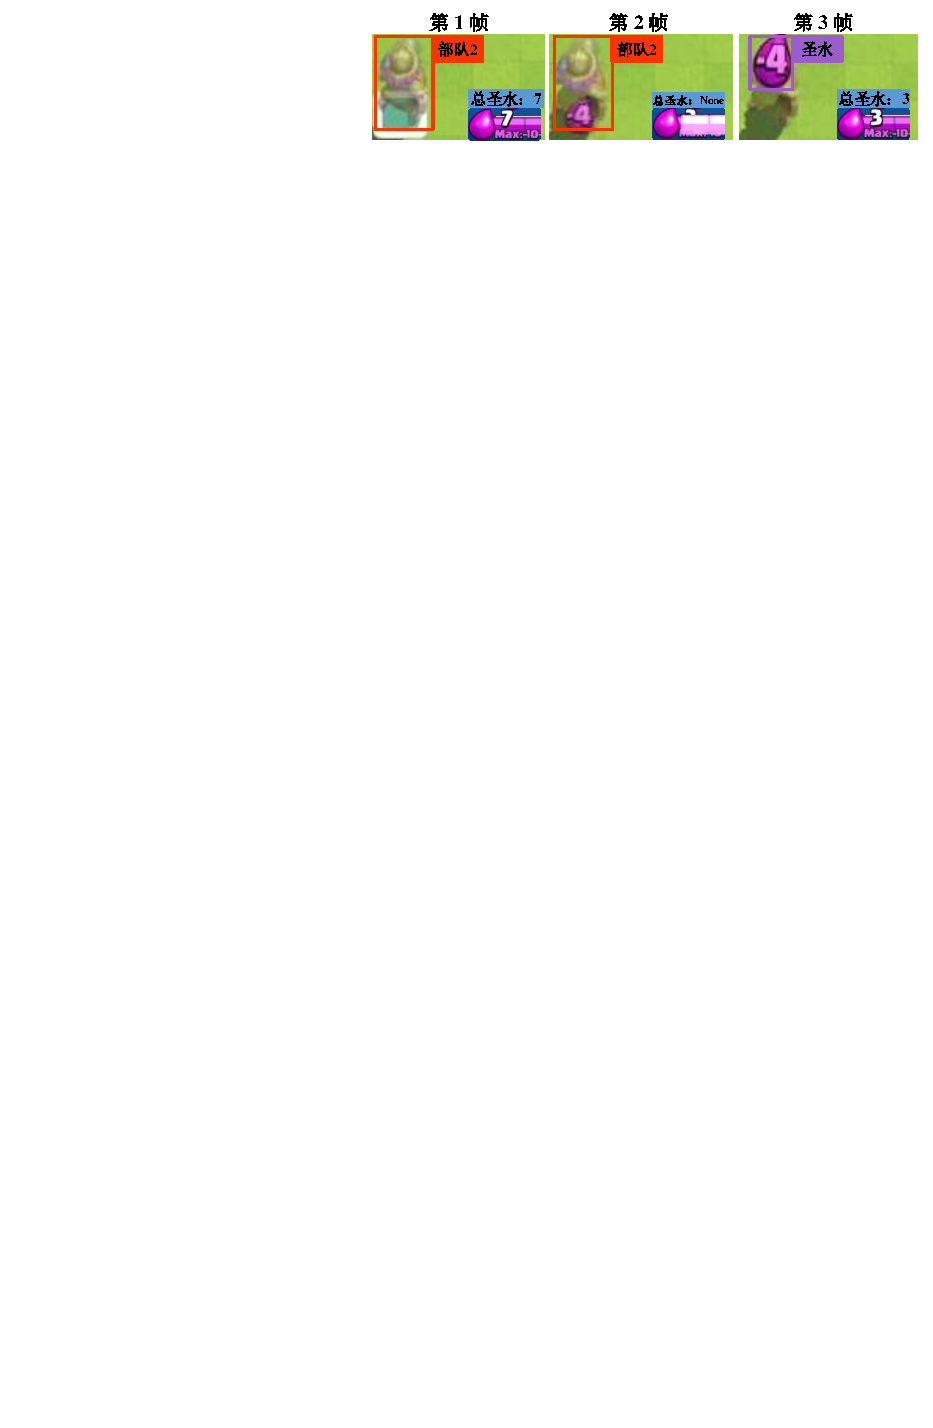
\includegraphics[width=0.8\textwidth]{state_and_action.pdf}
  \vspace{4ex}
  \caption{动作直接导致的错误状态先验信息:第1帧中目标识别错误识别到未部署的部队状态;
  第2帧中OCR识别器在目标识别识别到动作之前,产生了错误的总圣水识别信息,因此需要将动作帧提前到该帧之前;
  第3帧中目标识别成功识别到圣水动画,可以判断玩家在该时刻之前部署了部队。}
  \label{fig-state-action}
\end{figure}
% \begin{wrapfigure}[11]{r}{.6\textwidth} % 文字环绕行数为13行, 图片靠右 (l为靠左), 图片占0.5的行宽
%   \centering
%   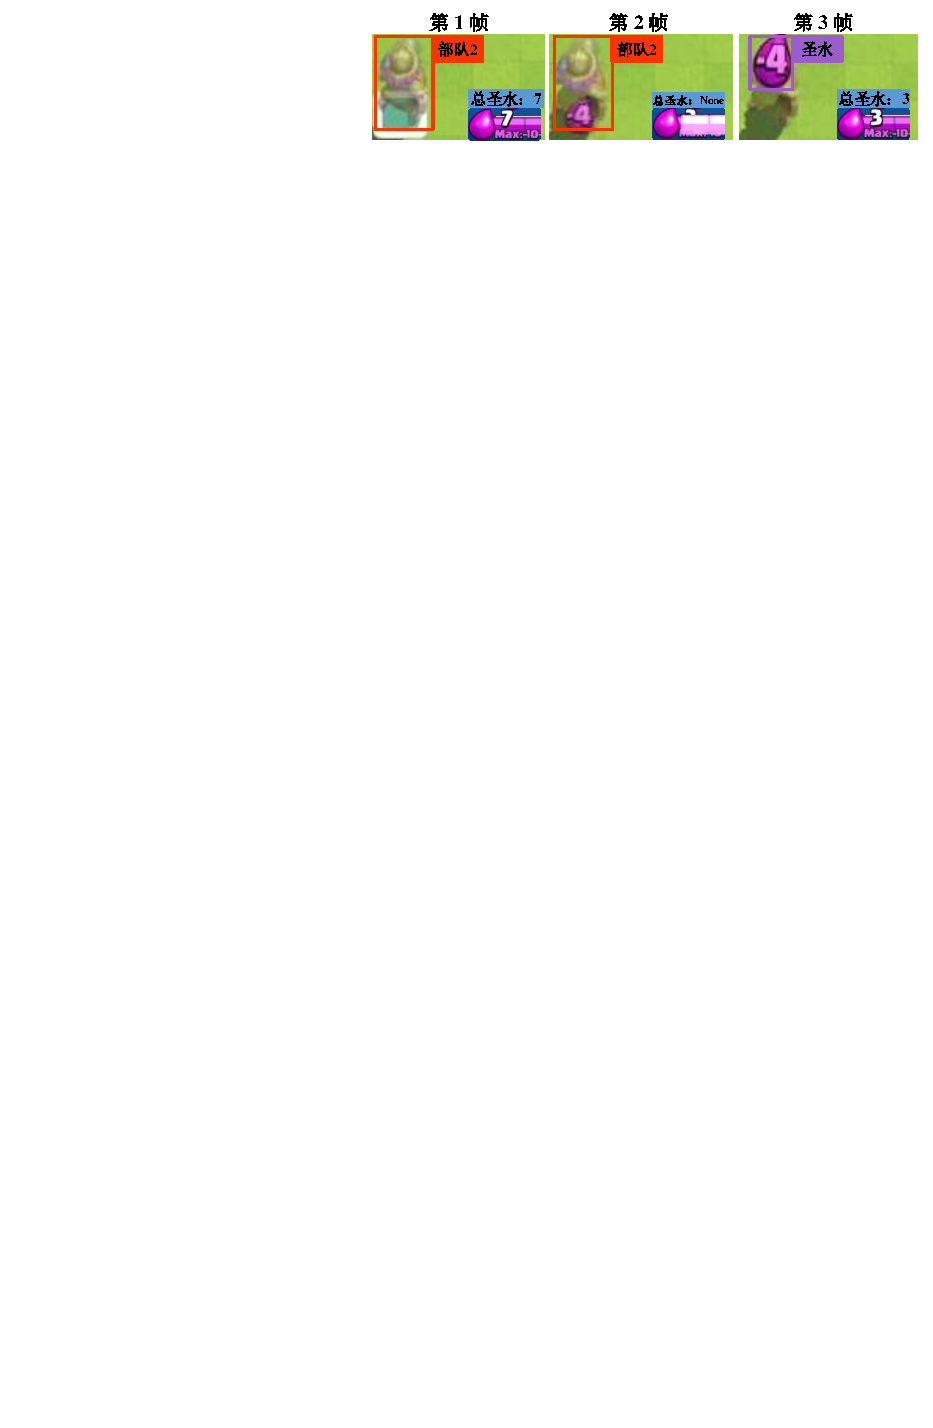
\includegraphics[width=.6\textwidth]{state_and_action.pdf}
%   \caption{动作直接导致的错误状态先验信息:第1帧中目标识别错误识别到未部署的部队状态;
%   第2帧中OCR识别器在目标识别识别到动作之前,产生了错误的总圣水识别信息,因此需要将动作帧提前到该帧之前;
%   第3帧中目标识别成功识别到圣水动画,可以判断玩家在该时刻之前部署了部队。}
%   \label{fig-state-action}
% \end{wrapfigure}

需要注意状态处理的细节问题,在执行动作之前,状态特征中应不包含任何直接与该动作相关的先验信息,
否则模仿学习可以通过该先验信息直接给出动作预测,而真实环境中由于不再出现这类动作的先验信息,
所以导致模型无法做出决策,错误状态信息如右图~\ref{fig-state-action}~所示。

假设目标识别每个预测框的识别结果包括七个参数$b:=(x,y,w,h,\text{id},\text{cls},\text{bel})$,
分别为预测框的中心点$(x,y)$,宽高$(w,h)$,目标追踪编号id,预测所属类别cls以及所属派别bel。

\begin{definition}[计数记忆缓存]
  设$I\subset \mathbb{N}$为目标追踪指标集,$S$为可数记忆元素集合,$V\subset \mathbb{R}^+$为可用时间集合,
  定义$M_{T}:I\times S\to\mathbb{Z}^+\times V$为缓存大小为$T$的计数记忆缓存,其满足
  $\forall~ \text{id}\in I, s\in S, (n,t):=M_T(\text{id},s)$,在时间间隔$[t-T,t]\cap V$下追踪指标为id的预测框中,
  存在$n$个预测框包含元素$s$。
\end{definition}

初始化派别记忆缓存$M_{T}^{\text{bel}}$和类别记忆缓存$M_{T}^{\text{cls}}$,其记忆元素集合分别为派别集合$\{0,1\}$
及全体类别集合,假设当前时间为$t$,于是状态特征提取可以分为下述6步\footnote{状态特征提取代码框架见附录~\ref{app-state-feature}~。}:

1. 更新派别记忆缓存:对当前每个预测框$b$,更新$M_{T}^{\text{bel}}(b^{\text{id}}, b^{\text{bel}})$,并对$b^{\text{bel}}$进行修正,
使得$M_T^{\text{bel}}(b^{\text{id}}, b^{\text{bel}})_1 = \max\left\{M_T^{\text{bel}}(b^{\text{id}},x)_1:x\in\{0,1\}\right\}$。

2. 全局文本信息查找:使用OCR对当前竞技场中全部文本信息进行识别,用于解决图~\ref{fig-state-action}~中未放置单位的错误识别问题。

3. 等级、生命值及防御塔信息关联:将等级与部队生命值、防御塔与防御塔生命值进行关联。

4. 部队信息关联:基于贪心的关联策略,从下至上,将部队与在一定范围内最近的等级和生命值进行关联,并基于步骤2结果,去除具有对应文本的部队单位。

5. 缓存清理:将$M_T^{\text{bel}},M_T^{\text{cls}}$中超出时间间隔$[t-T,t]$的信息置零。

6. 更新类别记忆缓存:结合关联性信息,对部队及其关联的等级和生命值信息所对应的$M_T^{\text{cls}}$进行更新,同时对部队类别进行修正,
更新及修正方法与步骤1类似。

\BiSubsection{动作特征提取}{}\label{sub-sec-action}
动作特征包含两种信息:
\begin{itemize}
  \item 当前执行动作的二维坐标$\bd{x}$。
  \item 当前执行动作所用的卡牌编号$\text{card}\in\{1,2,3,4\}$。
\end{itemize}

在进行动作特征提取时,需通过目标识别模型识别到的圣水预测框来判断执行动作的时刻以及坐标位置,
对圣水预测框的目标检测如图~\ref{fig-state-action}~中第3帧所示,但是在第2帧中已经出现了圣水对象,
动作执行本应该发生在第2帧,但是模型无法对其进行识别导致动作判断出现延迟,
所以需通过第2帧中总圣水识别发生突变来进行判断动作的执行,因此需要将第3帧识别到的动作前移至第2帧上。

还需结合当前手牌及圣水上方的文字信息来判断使用的卡牌编号,通过维护一个手牌记忆缓存记录当前可用手牌,
当手牌被玩家或智能体拖出牌库,则将其加入到候选手牌中,每次动作执行的卡牌编号将文本与候选手牌进行比对得到,
当两个文本串的Levenshtein编辑距离\upcite{LevenshteinDistance}不超过2时,则认为两个文本串相同。

初始化圣水记忆缓存$M_{T}^{\text{elixir}}$,其记忆元素集合为可部署单位的二维坐标空间,假设当前时间为$t$,
于是动作特征提取可以分为下述4步\footnote{动作特征提取代码框架见附录~\ref{app-action-feature}~。}:

1. 缓存清理:将$M_{T}^{\text{elixir}}$中超出时间间隔$[t-T,t]$的信息置零。

2. 更新可用手牌及候选手牌:通过手牌分类器的识别结果以及缓存中记录的手牌,可以完成候选手牌、可用手牌的信息更新。

3. 记录总圣水的突变时刻:通过OCR识别当前总圣水以及上一帧总圣水,可用判断当前的总圣水是否发生减少或者无法识别的情况,
当此类情况发生则认为动作执行可能发生在当前帧。

4. 动作查找:通过竞技场中对圣水单位的目标识别,判断动作执行的位置,动作执行的真实时刻为一段时间内最早发生的总圣水突变时刻,
动作卡牌编号需要结合OCR文本识别与候选手牌集合判断,最后再对当前可用手牌进行更新。
\BiSubsection{奖励特征提取}{}
奖励特征仅包含奖励$r\in\mathbb{R}$一种信息,通过OCR识别可以得到敌我防御塔具体生命值,敌我主、副塔如图~\ref{fig-introduction}~中所示,
设$h_{i}^{\text{bel}}, (i\in\{0,1,2\},\text{bel}\in\{0,1\})$为防御塔生命值,
当$i=1,2$时表示左右两个副塔生命值,$i=0$表示主塔生命值,$\text{bel}=0,1$分别表示我方和敌方建筑,
$\Delta h_{i}^{\text{bel}}$表示前一帧与当前帧生命值的差值,$H_{i}^{\text{bel}}$表示对应防御塔的总生命值,分别定义如下四种奖励函数:

1. 防御塔生命值奖励
\begin{equation}
  r_{tower} = \sum_{\text{bel}=0}^1\sum_{i=0}^2(-1)^{\text{bel}+1}\frac{\Delta h_{i}^{\text{bel}}}{H_{i}^{\text{bel}}}
\end{equation}

2. 防御塔摧毁奖励$r_{distory}$:当敌我副塔被摧毁时给予$(-1)^{\text{bel}+1}$奖励,敌我主塔被摧毁时给予前者的$3$倍奖励。

3. 主塔激活奖励$r_{activate}$:当副塔均存活的条件下,主塔第一次失去生命值时,给予$(-1)^{\text{bel}}~0.1$奖励。

4. 圣水溢出惩罚$r_{elixir}$:当总圣水持续保持溢出状态时,每间隔$1$秒产生一次$0.05$的惩罚。

综合上述奖励,得到总奖励\footnote{奖励特征提取代码框架见附录~\ref{app-reward-feature}~。}:
\begin{equation}\label{eq-reward}
  r = r_{tower} + r_{destory} + r_{activate} + r_{elixir}
\end{equation}

需要注意的是,当图像中的数字信息出现噪声干扰或产生错误目标位置识别时,需要终止奖励的错误更新,
例如:部署单位时其他部件对其产生的遮挡(等级、生命值、圣水、时钟、文本)。

\BiSection{决策模型}{}\label{sec-model}
\BiSubsection{离线强化学习}{}\label{sec-offline-rl}
离线强化学习(Offline Reinforcement Learning)是指在没有与环境交互的情况下,
使用预先收集的随机或专家数据来训练强化学习算法,这类算法适用于无法频繁与环境交互或交互代价高昂的场景,
例如自动驾驶、机器人控制等。由于本任务中的非嵌入环境,与环境交互速度效率很低,所以考虑使用离线强化学习作为决策模型。

首先对强化学习中的概念进行介绍,
考虑无限长带折扣Markov决策过程(Markov Decision Process, MDP),定义为$(\mathcal{S},\mathcal{A},p,r,\gamma)$,
其中$\mathcal{S}$为状态空间,$\mathcal{A}$为动作空间,
$p:\mathcal{S}\times \mathcal{A}\times \mathcal{S}\to \mathbb{R}$为状态转移方程,
$r:\mathcal{S}\times\mathcal{A}\to \mathbb{R}$为奖励函数,$\gamma\in(0,1)$为折扣系数。
令$\pi$表示决策函数$\pi: \mathcal{S}\times \mathcal{A}\to [0,1]$,令$R(\pi)$表示其期望所获得的总奖励(回报):
\begin{equation}
  R(\pi) = \mathbb{E}_{S_1,A_1,S_2,A_2\cdots}\left[\sum_{t=0}^{\infty}r(S_t,A_t)\right],\quad
  \text{~其中~}A_t\sim\pi(\cdot|S_t),S_{t+1}\sim p(\cdot|s_t,a_t)
\end{equation}
强化学习的目标通常是找到最优策略$\pi^* := \argmax_{\pi}R(\pi)$,
在线强化学习算法往往通过策略迭代和价值函数估计方法实现策略的更新,
而下文中所使用的离线强化学习算法不再基于值估计方法,而是更加类似于模仿学习的方法。

Decision Transformer(DT)\upcite{DT}是一种将强化学习问题是为序列建模问题的方法,使用了深度学习中的Transformer架构,
对于离线数据集中的一段长度为$T$的交互轨迹(Trajectory)
\begin{equation}
  \rho = (s_1,a_1,r_1,s_2,a_2,r_2,\cdots,s_T,a_T,r_T,s_{T+1})
\end{equation}
其中$s_{T+1}$为终止状态,则$\rho$可以视为建模为序列
\begin{equation}\label{eq-sequence}
  R_0,s_1,a_1,R_1,s_2,\cdots,a_{T-1},R_{T-1},s_{T},a_{T}
\end{equation}
其中$R_i=\sum_{t=i}^Tr_{t+1}, (i=0,\cdots,T-1)$为目标回报(Return-to-Go)。

DT模型中序列编码模型使用的是GPT模型\upcite{GPT},即仅含有编码器的因果注意力机制。
具体来讲,假设当前处理的序列$X\in\mathbb{R}^{d\times N}$长度为$N$,每个特征编码维度为$d$,
则注意力机制\upcite{attention}包含三个可学习矩阵$W_{Q},W_{K}\in\mathbb{R}^{d_k\times d}, W_{V}\in\mathbb{R}^{d_v\times d}$,
分别对应生成询问键(Query),查询键(Key)和价值键(Value)
\begin{equation}
  \left\{
  \begin{aligned}
  Q=&\ W_{Q}X\\ K=&\ W_{K}X\\ V=&\ W_{V}X
  \end{aligned}
  \right.
\end{equation}
则对于序列中第$i\in\{1,\cdots,N\}$个特征对应的交叉注意力(Cross-Attention)为
\begin{equation}
  \bd{z}^{cross}_i = \sum_{j=1}^N\text{softmax}\left(\left\{\frac{1}{\sqrt{d_k}}\langle \bd{q}_i,\bd{k}_l\rangle\right\}_{l=1}^N\right)_j\cdot \bd{v}_j\iff
  Z^{cross} = \text{softmax}\left(\frac{QK^T}{\sqrt{d_k}}\right)V
\end{equation}
其中包含系数$1/\sqrt{d_k}$的原因:不妨假设$\bd{q}_{ij}\bd{k}_{lj}\sim \mathcal{N}(0,\sigma^2),~(j\in\{1,\cdots,d_k\})$,
则$\sum_{j=1}^{d_k}\bd{q}_{ij}\bd{k}_{lj}\sim\mathcal{N}(0,d_k\sigma^2)$,由于初始化的神经网络输出可以保证$\sigma\approx 1$,
因此使用系数$1/\sqrt{d_k}$可以保持输出的方差在$1$左右,避免发散。

因果注意力(Causal-Attention)为(每个特征$i$只能看到$j\leqslant i$的特征)
\begin{equation}\label{eq-causal-attn}
\begin{aligned}
  &\ \bd{z}^{causal}_i = \sum_{j=1}^i\text{softmax}\left(\left\{\frac{1}{\sqrt{d_k}}\langle \bd{q}_i,\bd{k}_l\rangle \right\}_{l=1}^N\right)_j\cdot \bd{v}_j\\
  \iff &\ Z^{causal} = \text{softmax}\left(\frac{\left(QK^T\right)\odot M}{\sqrt{d_k}}\right)V
\end{aligned}
\end{equation}
其中$M$为$N$阶下三角阵,引入因果注意力机制后,每个特征由于无法观察到后续特征,所以可以对相邻的下一个特征进行预测,
从而无需再对编码器和解码器进行区分,降低了代码复杂性。

DT训练方法:首先从离线数据集中随机采样得到一段长度为$N$的轨迹
\begin{equation}
  \tau_{t-N+1:t} =: (R_0,s_1,a_1,R_1,s_2,a_2,\cdots,R_{N-1},s_N,a_N) = \{R_{n-1},s_n,a_n\}_{n=1}^N
\end{equation}

将每个特征编码到相同维度$\mathbb{R}^d$下,按式~(\ref{eq-sequence})
建模为长度$3N$的序列$\tau\in\mathbb{R}^{3N\times d}$,用GPT模型对序列进行特征编码可以得到和$\tau$维度相同的编码序列$\tau'$,
再取出状态序列所对应的编码结果,通过线性变换映射到动作空间维度,从而得到对相邻动作的预测
\begin{equation}
  (\tau'_2,\tau'_5,\cdots, \tau'_{3N-1})\xrightarrow{\text{~线性变换~}}
  (\hat{a}_1,\hat{a}_2,\cdots,  \hat{a}_{N})
\end{equation}

对于离散动作空间使用多元交叉熵损失,连续动作空间则使用$\ell^2$范数(Mean Square Error, MSE)作为损失函数。

DT验证方法:需给出模型期望达到的总奖励$\hat{R}_0$,通过自迭代的方式使模型完成动作预测,
具体来说,假设初始状态为$s_1$,则初始轨迹为$\tau_1=(\hat{R}_0,s_1)$,模型对$\tau_1$进行编码,
取出最后一个状态$s_1$所对应的预测动作$\hat{a}_1$与环境交互,
得到新的状态$s_2$和奖励$r_1$,令$\hat{R}_1 = \hat{R}_0 - r_1$,
从而得到新的序列$\tau_2 = (\hat{R}_0,s_1,\hat{a}_1, \hat{R}_1, s_2)$,模型再对$\tau_2$进行编码,
取出$s_2$所对应的预测动作$\hat{a}_2$与环境交互,以此类推,直到环境达到终止状态为止。
这种方式和自然语言模型中文本生成的做法基本一致。

StARformer\upcite{StARformer}是一种基于ViT\upcite{ViT}专门对状态中的图像特征编码进行的改进,
通过将轨迹$\tau$中的$\{(a_{n-1},R_{n-1},s_{n})\}_{n=1}^{3N}$($a_0$使用特征填充补全)
按照空间维度进行展开($s_{n}$使用ViT中图像分块的方法将图像分块序列化),
并压缩到空间特征维度$d'$,进而在空间维度上使用交叉注意力机制进行编码,
得到$\{a'_{n-1},R'_{n-1},s'_{n}\}_{n=1}^{3N}$,
再将第$n$时刻对应的编码$(a'_{n-1},R'_{n-1},s'_{n})$全部展平,
使用线性变换到时间维度$\mathbb{R}^d$中,将其记为$\{l_{n}\}_{n=1}^N$,
则时间维度的序列建模为
\begin{equation}
  \tau:=s_1,l_1,s_2,l_2,\cdots,s_N,l_N
\end{equation}

通过因果注意力机制(相邻的$(s_n,l_n),~n=1,\cdots,N$之间仍然具有注意力机制)可以完成对时序序列信息的编码,
将编码结果记为$\tau'$,
类似DT的预测方法,只考虑所有状态对应的编码结果,
通过线性变换映射到动作空间维度,从而得到相邻动作的预测
\begin{equation}
  (\tau'_1,\tau'_3,\cdots, \tau'_{2N-1})\xrightarrow{\text{~线性变换~}}
  (\hat{a}_1,\hat{a}_2,\cdots, \hat{a}_{N})
\end{equation}
模型的训练及推理方式与DT完全一致,相比DT模型,StARformer能够有效的提高模型对图像信息的理解能力,
本毕设对上述离线强化学习算法进行了复现\footnote{\url{https://github.com/wty-yy/Decision-Transformer-JAX},
复现内容包括:Decision Transformer(DT),Return-Aligned Decision Transformer(RADT)和StARformer,
在Atari环境中进行了对比试验,并对结果进行可视化。在5个不同Atari环境下的实验表明,StARformer的平均得分超过DT算法的$30\%$。},本文的相关复现实验显示
相比DT更不依赖于初始时目标总奖励$\hat{R}_0$的设定,这说明其更倾向于对专家数据的模仿学习,而非与目标总奖励进行对齐。

\BiSubsection{状态空间与动作空间}{}
模型的状态输入由2部分构成,分别为$S^{img}, \bd{s}^{card}$,其中$S^{img}\in\mathbb{R}^{18\times 32\times 15}$为单位的网格状特征输入,
对于第$i$行$j$列的特征$\bd{z}_{ij}:=(S^{img})_{ij}\in\mathbb{R}^{15}$
表示处于该位置的单位具有如下$4$种特征:$(\bd{z}_{ij})_{1:8}$为类别编码,
$(\bd{z}_{ij})_9$为从属派别编码,$(\bd{z}_{ij})_{10:12}$为生命值图像编码,$(\bd{z}_{ij})_{13:15}$为其余条状图像编码;
$\bd{s}^{card}\in\mathbb{R}^6$表示当前状态下的两个全局特征:$(\bd{s}^{card})_{1:5}$为当前手牌信息,
$(\bd{s}^{card})_6$为当前总圣水量。

模型的动作输入由2个部分构成:$\bd{a}^{pos}, a^{select}$,其中$\bd{a}^{pos}\in\mathbb{R}^2$表示动作执行的部署坐标,
$a^{select}$表示动作执行的手牌编号。

\BiSubsection{预测目标设计与重采样}{}\label{sec-target}
由于本任务中动作执行极为离散,总帧数中仅有$4\%$为执行动作帧,其余帧均不执行动作,
如果直接逐帧预测动作会产生非常严重的长尾问题,导致模型最终基本不执行动作(表~\ref{table-model-eval}~中离散预测的动作数远低于连续动作预测数),
因此需要将预测目标从离散转化为连续,解决方法是引入延迟动作预测:
对于第$i$帧,需找到其后(包含自身)最近的动作帧$j$,令最大间隔帧数阈值为$T_{delay}$,
则每个非动作帧的预测的延迟动作为$a^{delay}_{i} = \min\{j-i, T_{delay}\}$。

对离线数据集进行采样时,为避免长尾问题导致模型偏移,本文还设置了重采样频次,
设数据集总帧数为$N$,动作帧数为$N_{action}$,则动作帧占比为$r_a:=N_{action} / N$,
对于第$i$个动作帧位于数据集中的第$t_i$帧,则$j\in\{t_{i},\cdots,t_{i+1}-1\}$帧作对应的重采样频次为
\begin{equation}\label{eq-resample-freq}
  s_j = \max\left\{\frac{1}{1-r_a}, \frac{1}{r_a(j-t_i+1)}\right\},\quad (t_i\leqslant j\leqslant t_{i+1})
\end{equation}
则训练轨迹中结束帧的采样分布为$\left\{\frac{s_j}{\sum_{j=1}^{N}s_j}\right\}_{j=1}^N$,
图~\ref{fig-resample-and-delay}~中展示了离线数据集一段轨迹所对应的重采样频次与动作预测值。
\begin{figure}[htbp]
  \centering
  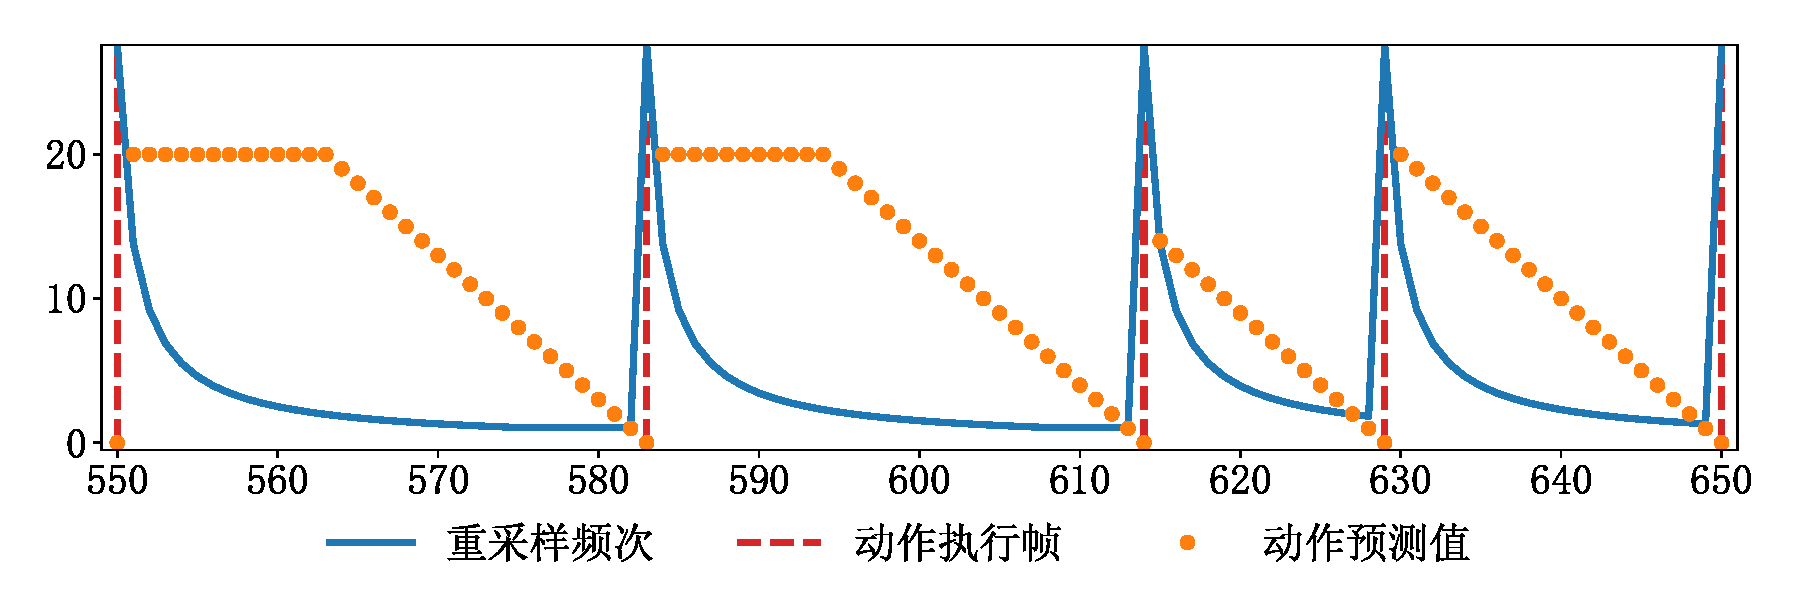
\includegraphics[width=\textwidth]{resample_and_delay.pdf}
  \caption{从离线数据集中截取的一段数据,总共包含5个动作帧,最大间隔帧数阈值$T_{delay} = 20$,}\label{fig-resample-and-delay}
\end{figure}

\BiSubsection{模型架构设计}{}\label{sec-model-struct}
\begin{figure}[htbp]
  \centering\vspace{-2ex}
  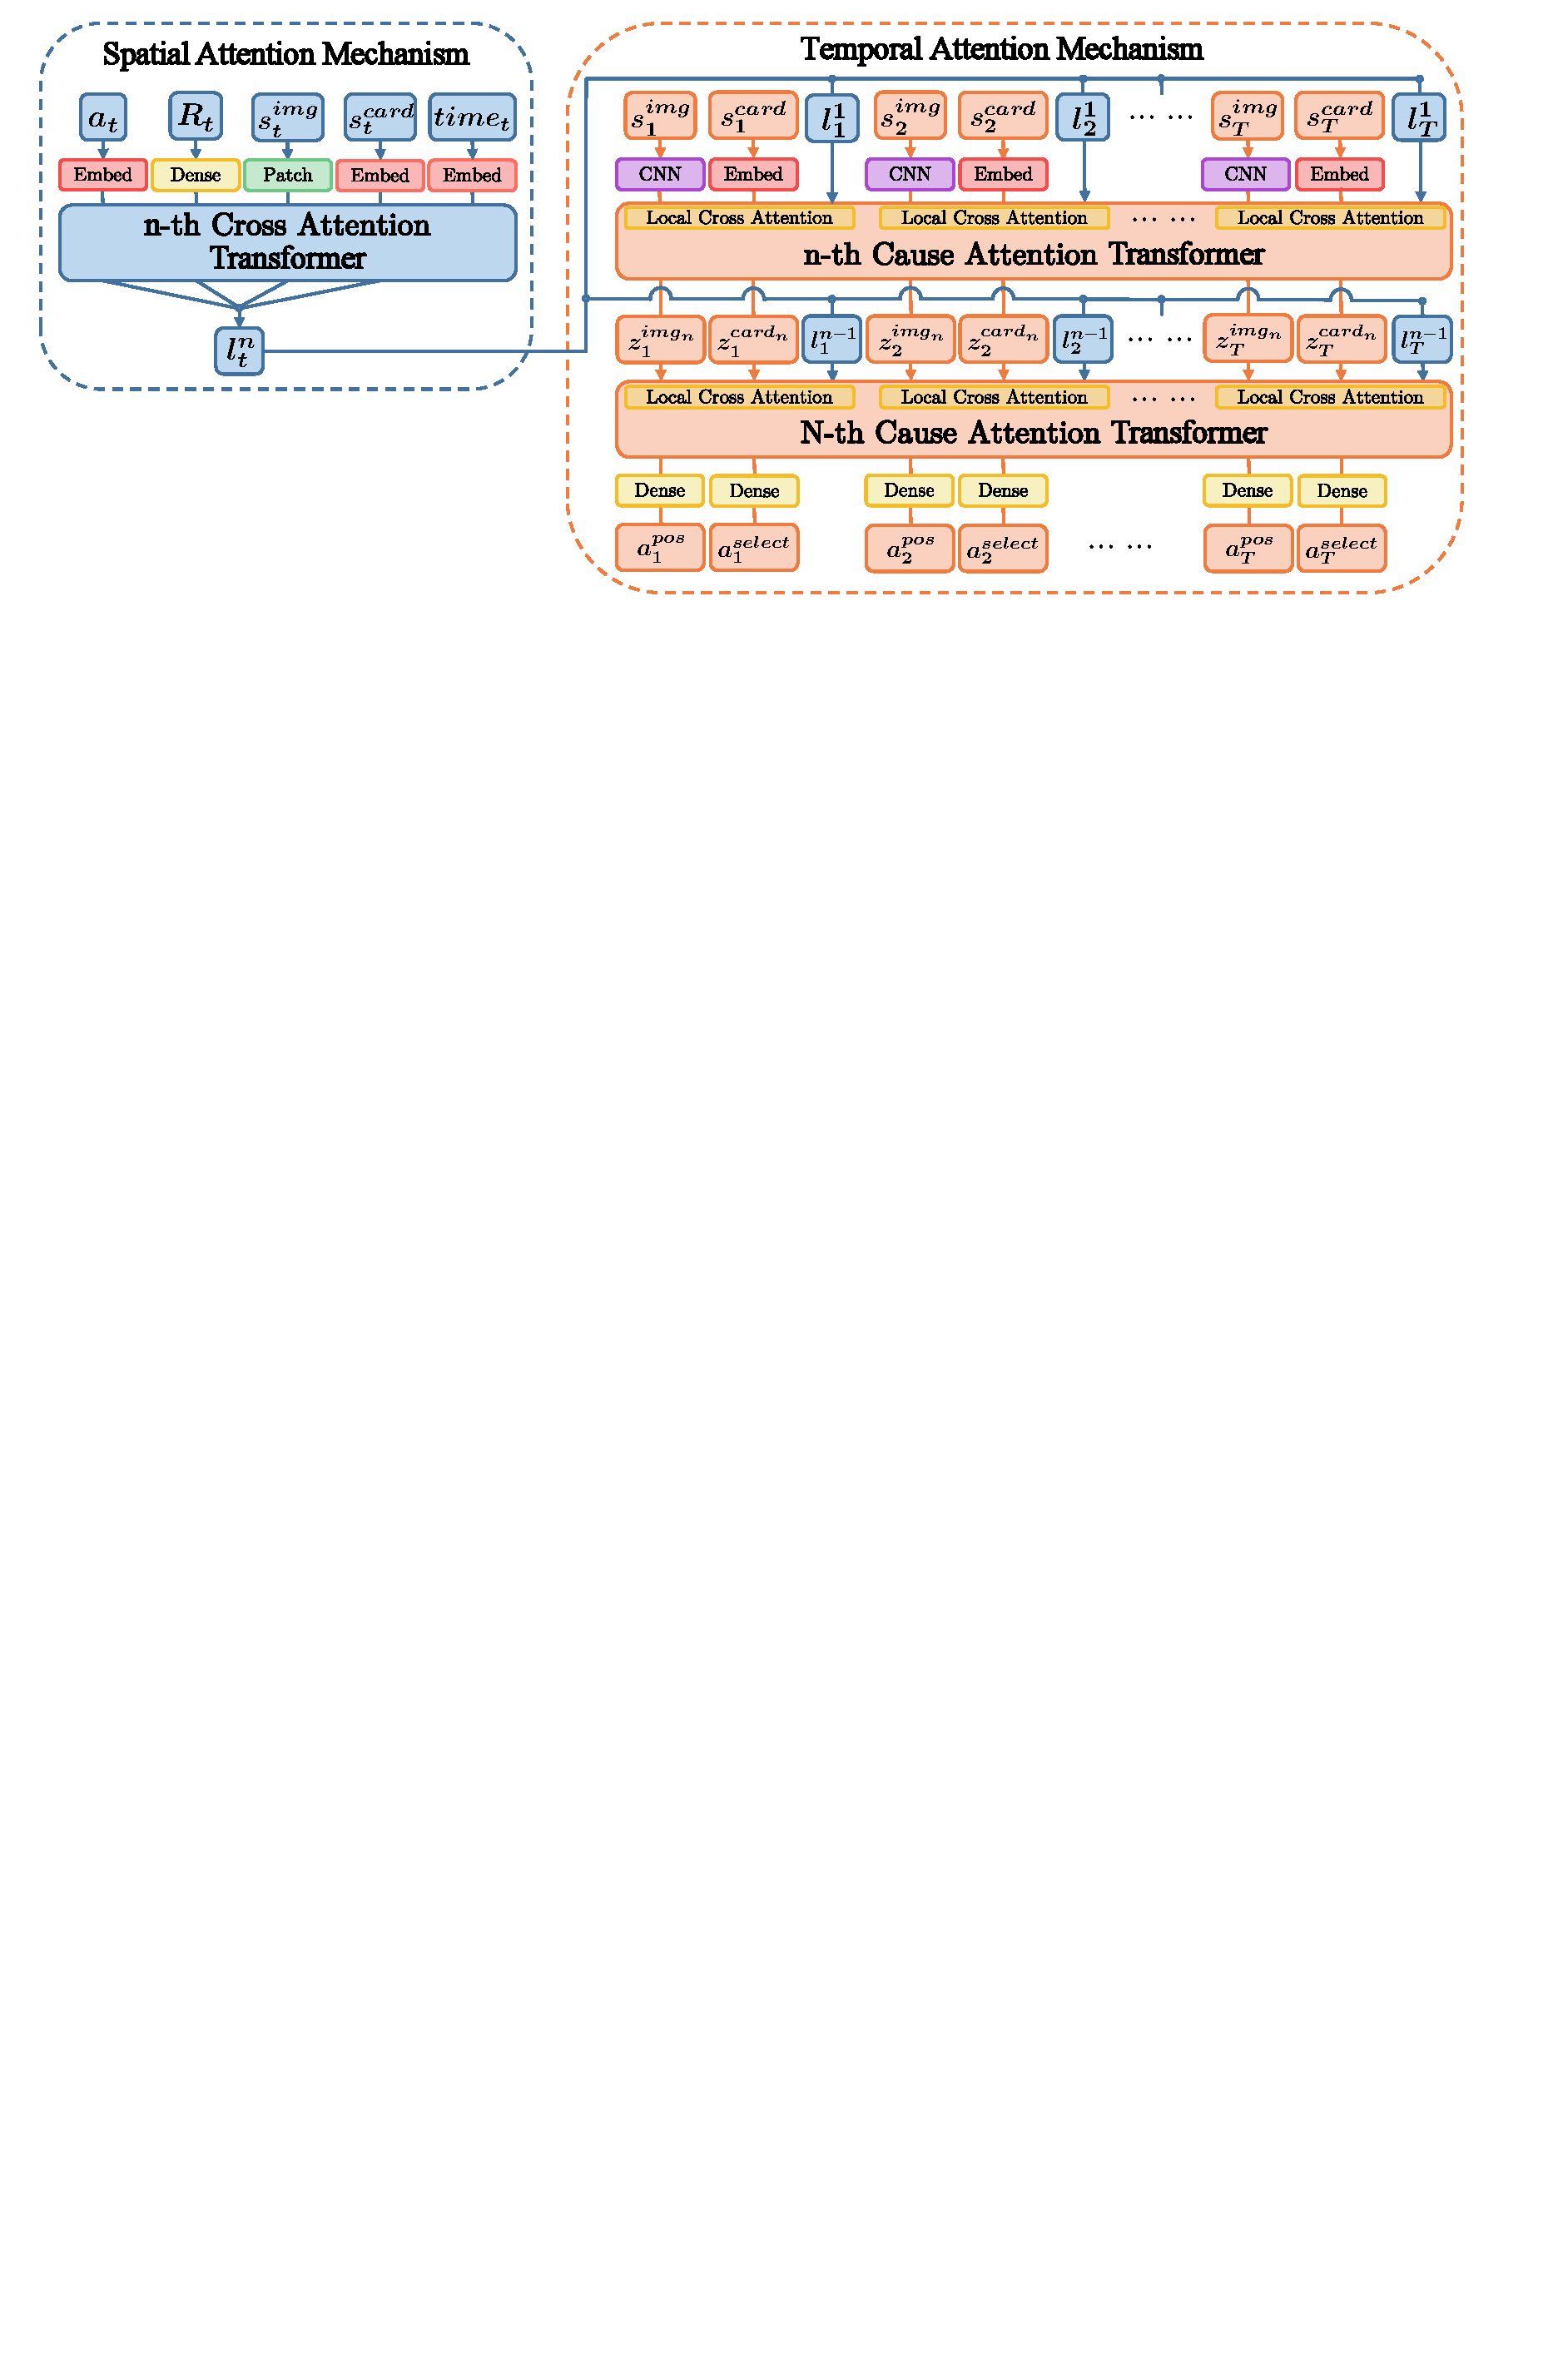
\includegraphics[width=\textwidth]{policy_model.pdf}
  \caption{决策模型架构}
  \label{fig-model}
\end{figure}

本文使用的决策模型架构如图~\ref{fig-model}~所示,基于StARformer的ViT+DT架构,模型输入为轨迹序列$(a_t, R_t, s_t)_{t=1}^T$,
输出为动作预测序列$(a_t^{pos},a_t^{select})_{t=1}^T$。左侧交叉注意力机制对
局部信息$(a_t,R_t,s_t)$按空间维度进行编码,并使用ViT中分块思路将图像$s_t^{img}$转化为序列;
右侧为因果注意力机制对全局信息$(s^{img}_t,s^{card}_t)$按时序维度进行编码,
并在每层序列输入中引入对应的局部编码信息$l_t^{n}$。

本文总共设计了3种不同的模型架构,分别基于StARformer和DT模型,
假设输入的轨迹长度为$L$,时序注意力机制中的输入序列长度$T$,使用$N$层Transformer堆叠,
则每种模型架构设计细节如下:

StARformer-3L:基于StARformer架构,
本文设计的StARformer-3L决策模型架构如图~\ref{fig-model}~所示,
其中输入序列长度$T=3L$,第$n$层Transformer输出的时序序列记为
$\{z_t^{img_n},z_t^{card_n},l_{t}^{n-1}\}_{t=1}^{L}$(序列长度$3L$)。
右侧时序注意力机制中的因果Transformer,由于需要使同一时刻下的信息可以相互产生注意力关系,
所以需要引入局部交叉注意力,具体实现方法是将式~(\ref{eq-causal-attn})~中的掩码矩阵$M_{3}$,其中$M_{L_0}$定义为
\begin{equation}
  (M_{L_0})_{ij} = \begin{cases}
    1, &\quad i=kL_0-l,j\leqslant kL_0\\
    0, &\quad \text{否则}
  \end{cases},\quad k\in\{1,\cdots,L\}, l\in\{0,\cdots,L_0-1\}
\end{equation}
其本质上是在下三角阵的对角线上顺次放置不交的大小为$L_0\times L_0$的全$1$矩阵。

StARformer-2L:$T=2L$的模型架构与StARformer\upcite{StARformer}论文中架构基本一致,其将图像信息$s_{t}^{img}$与$s_{t}^{card}$编码到同一特征$z_t$中,
得到第$n$层的Transformer输出的时序序列$\{z_t^{n}, l_{t}^{n-1}\}_{t=1}^{L}$(序列长度$2L$),
同理需要使用局部交叉注意力,并将掩码矩阵置为$M_2$,
预测中$a_{t}^{pos}$和$a_{t}^{select}$均使用$z_t$进行解码得到。

DT-4L:基于DT架构,可以看作仅包含图~\ref{fig-model}~中时序注意力部分,
将时序注意力机制中$l_t^{n}$进行替换,得到时序序列为$\{a_{t-1},R_{t-1},s_{t}^{img_n}, s_{t}^{card_n}\}_{t=1}^{L}$(序列长度$4L$),
预测中$a_{t}^{pos}$和$a_{t}^{select}$分别由$s_{t}^{img_n}$和$s_{t}^{card_n}$对应解码得到。

% \BiSection{感知融合小结}{}
% 
% \BiChapter{决策模型}{4}\label{chpt-4}
% 本章首先对离线强化学习中的传统模型进行介绍,再给出本文对模型架构及预测目标的改进内容,
% 相关实验结果在~\ref{sec-decision-model}~中展示。
\BiSection{本章小结}{}
感知融合:首先分别对YOLO系列目标识别模型、PaddleOCR光学字符识别模型、ResNet图像分类器进行介绍,将其作为非嵌入图像特征信息的初步提取器,
再通过状态、动作、奖励三种不同感知特征提取器对特征信息进行融合,通过结合上下帧信息及单位的关联信息恢复漏识别目标,
排除对动作决策具有干扰的特征,最后将融合完成的特征作为~\ref{sec-model}~中决策模型的输入信息。

决策模型:先对离线强化学习中的基本定义及DT和StARformer模型进行介绍,详细介绍了训练及推理的实现方法。
由于本任务的离线数据集中存在严重的长尾问题,
本文通过对预测目标的重新设计,并在模型训练中加入重采样策略,从而一定程度上缓解了长尾问题。
最后本文还对StARformer模型架构做出了改进,设计了三种不同的决策模型框架,进行对比实验测试(见表~\ref{table-model-eval})。
从表中可知,预测目标修改提高了$37\%$的模型性能,
将StARformer模型架构从2L修改为3L提高了$24\%$的模型性能。
